\documentclass[]{elsarticle} %review=doublespace preprint=single 5p=2 column
%%% Begin My package additions %%%%%%%%%%%%%%%%%%%
\usepackage[hyphens]{url}

  \journal{The Journal of Mass Spectrometry:Applications to the Clinical
Laboratory} % Sets Journal name


\usepackage{lineno} % add
\providecommand{\tightlist}{%
  \setlength{\itemsep}{0pt}\setlength{\parskip}{0pt}}

\usepackage{graphicx}
\usepackage{booktabs} % book-quality tables
%%%%%%%%%%%%%%%% end my additions to header

\usepackage[T1]{fontenc}
\usepackage{lmodern}
\usepackage{amssymb,amsmath}
\usepackage{ifxetex,ifluatex}
\usepackage{fixltx2e} % provides \textsubscript
% use upquote if available, for straight quotes in verbatim environments
\IfFileExists{upquote.sty}{\usepackage{upquote}}{}
\ifnum 0\ifxetex 1\fi\ifluatex 1\fi=0 % if pdftex
  \usepackage[utf8]{inputenc}
\else % if luatex or xelatex
  \usepackage{fontspec}
  \ifxetex
    \usepackage{xltxtra,xunicode}
  \fi
  \defaultfontfeatures{Mapping=tex-text,Scale=MatchLowercase}
  \newcommand{\euro}{€}
\fi
% use microtype if available
\IfFileExists{microtype.sty}{\usepackage{microtype}}{}
\bibliographystyle{elsarticle-harv}
\ifxetex
  \usepackage[setpagesize=false, % page size defined by xetex
              unicode=false, % unicode breaks when used with xetex
              xetex]{hyperref}
\else
  \usepackage[unicode=true]{hyperref}
\fi
\hypersetup{breaklinks=true,
            bookmarks=true,
            pdfauthor={},
            pdftitle={Continuous Reference Intervals for Pediatric Testosterone, Sex Hormone Binding Globulin and Free Testosterone using Quantile Regression},
            colorlinks=false,
            urlcolor=blue,
            linkcolor=magenta,
            pdfborder={0 0 0}}
\urlstyle{same}  % don't use monospace font for urls

\setcounter{secnumdepth}{5}
% Pandoc toggle for numbering sections (defaults to be off)

% Pandoc citation processing
\newlength{\csllabelwidth}
\setlength{\csllabelwidth}{3em}
\newlength{\cslhangindent}
\setlength{\cslhangindent}{1.5em}
% for Pandoc 2.8 to 2.10.1
\newenvironment{cslreferences}%
  {}%
  {\par}
% For Pandoc 2.11+
\newenvironment{CSLReferences}[3] % #1 hanging-ident, #2 entry spacing
 {% don't indent paragraphs
  \setlength{\parindent}{0pt}
  % turn on hanging indent if param 1 is 1
  \ifodd #1 \everypar{\setlength{\hangindent}{\cslhangindent}}\ignorespaces\fi
  % set entry spacing
  \ifnum #2 > 0
  \setlength{\parskip}{#2\baselineskip}
  \fi
 }%
 {}
\usepackage{calc} % for calculating minipage widths
\newcommand{\CSLBlock}[1]{#1\hfill\break}
\newcommand{\CSLLeftMargin}[1]{\parbox[t]{\csllabelwidth}{#1}}
\newcommand{\CSLRightInline}[1]{\parbox[t]{\linewidth - \csllabelwidth}{#1}}
\newcommand{\CSLIndent}[1]{\hspace{\cslhangindent}#1}

% Pandoc header
\usepackage{float}
\usepackage{url}
\usepackage{caption}
\usepackage{booktabs}
\usepackage{longtable}
\usepackage{array}
\usepackage{multirow}
\usepackage{wrapfig}
\usepackage{float}
\usepackage{colortbl}
\usepackage{pdflscape}
\usepackage{tabu}
\usepackage{threeparttable}
\usepackage{threeparttablex}
\usepackage[normalem]{ulem}
\usepackage{makecell}
\usepackage{xcolor}



\begin{document}
\begin{frontmatter}

  \title{Continuous Reference Intervals for Pediatric Testosterone, Sex
Hormone Binding Globulin and Free Testosterone using Quantile
Regression}
    \author[SPH,UBC]{Daniel T. Holmes\corref{1}}
   \ead{dtholmes@mail.ubc.ca} 
    \author[SPH]{J Grace van der Gugten\corref{1}}
   \ead{gvandergugten@providencehealth.bc.ca} 
    \author[HSC]{Benjamin Jung}
   \ead{benjamin.jung@sickkids.ca} 
    \author[UO,TOH,EORLA]{Christopher R. McCudden}
   \ead{cmccudde@uottawa.ca} 
      \address[SPH]{St.~Paul's Hospital Department of Pathology and
Laboratory Medicine, 1081 Burrard St., Vancouver, BC V6Z 1Y6 Canada}
    \address[UBC]{University of British Columbia Department of Pathology
and Laboratory Medicine, 2211 Wesbrook Mall, Vancouver, BC V6T 1Z7
Canada}
    \address[TOH]{Department of Pathology and Laboratory Medicine,
Ottawa Hospital, General Campus, 501 Smyth Road, Ottawa, ON K1H 8L6
Canada}
    \address[UO]{Department of Pathology and Laboratory Medicine,
University of Ottawa}
    \address[EORLA]{Eastern Ontario Regional Laboratory Association}
    \address[HSC]{Hospital for Sick Children (SickKids), 555 University
Ave., Department of Paediatric Laboratory Medicine, Toronto, ON, M5G
1X8}
      \cortext[1]{Corresponding Author}
  
  \begin{abstract}
  Testosterone (T), sex hormone binding globulin (SHBG), free
  testosterone (FT) and bioavailable testosterone (BAT) are commonly
  employed tests in pediatric endocrinology and all require
  age-dependent reference intervals for interpretation. The common
  methods used to derive these reference intervals require decisions
  about data shape and/or age partition thresholds, which can result in
  sharp differences between age groups, particularly for pubescent
  children. Partitioning also results in a form of data loss, where data
  from one age-bin is completed disconnected from the adjacent age-bins.
  Non-parametric continuous reference intervals methods have previously
  been developed to avoid some of these drawbacks. These strategies use
  all the available data and smooth transitions between ages avoiding
  partitioning. However, the fitting process inolves selection and
  adjustment of many parameters and it can be difficult to maintain a
  reproducible approach. Here we provide a workflow for non-parametric
  continuous reference intervals applied to T, FT, BAT, and SHBG using
  the R language quantregGrowth package. T measurements were determined
  by LC-MS/MS, FT and BAT were calculated, and SHBG was measured on the
  Roche Cobas e601. The continuous interval methodology is described in
  detail with code examples and illustrations for reproducibililty.
  \end{abstract}
  
 \end{frontmatter}

\hypertarget{introduction}{%
\section{Introduction}\label{introduction}}

Measurements of testosterone (T), sex hormone binding globulin (SHBG),
free testosterone (FT) and bioavailable testosterone (BAT) are common in
pediatric endocrinology for investigation of ambiguous genitalia,
precocious puberty, and premature adrenarche. Age-dependent reference
intervals for T, as measured by liquid chromatography and tandem mass
spectrometry (LC-MS/MS), have been previously investigated in a number
of studies using a number of statistical procedures including, the
Hoffmann method {[}1{]}, various partitioning strategies {[}2--6{]}, and
continuous fitting procedures {[}7{]}.

Statistical strategies for continuous fitting of age-dependent centiles
became a matter of interest for the development of pediatric growth
curves {[}8{]} but in time, these strategies have been applied to
age-dependent biochemical and hematological parameters. There are
numerous approaches to the problem, each addressing challenges of
heteroscedasticity and non-normality in the raw data in different ways.
Some of the more popular approaches include the those of Healy {[}8{]},
Cole's lambda, mu and sigma (LMS) method {[}9{]}, Royston's fractional
polynomial method {[}10{]}, the generalized additive models for
location, scale and shape (GAMLSS) method {[}11{]} and quantile
regression methods {[}12--14{]}

In this particular study we will demonstrate the application of the
non-parametric quantile regression method deployed in the
\textbf{quantregGrowth} package of the R programming language {[}15{]}.
This methodology will be applied to T, SHBG, calculated FT and
calculated BAT measured on a cohort of discarded anonymized samples from
421 children (195 F,226 M) aged 33 days to 19 years. We will illustrate
the process of performing such an analysis using the
\textbf{quantregGrowth} package.

\hypertarget{methods}{%
\section{Methods}\label{methods}}

\hypertarget{samples}{%
\subsection{Samples}\label{samples}}

Becton Dickenson and Greiner red top serum samples were obtained from
British Columbia Children's and Women's Hospital after routine analysis
for reactivity to allergens. After routine clinical analysis, specimens
were sequestered, anonymized and decanted to \(12\times 75\) mm
polystyrene tubes and frozen at -80 \(^{\circ}\)C. No clinical exclusion
criteria were applied to the cohort. These samples were then transferred
to St.~Paul's Hospital laboratory for the analysis of T and SHBG. SHBG
was measured within 2 months of receipt while T analysis was delayed for
3 years. Stability studies for SHBG have shown only modest changes at
-25 \(^{\circ}\)C for 25 years {[}16{]} while T is similarly unaffected
by years of storage at -80 \(^{\circ}\)C when measured by LC-MS/MS
{[}17{]}.

\hypertarget{biochemical-analysis}{%
\subsection{Biochemical Analysis}\label{biochemical-analysis}}

T analysis was performed using a modification French's method {[}18{]}
as previously described {[}19{]}. Briefly, liquid-liquid extraction was
performed on 100 µL of sample/calibrator with 40 µL of internal standard
(d3-testosterone at 11.7 nmol/L; 337 ng/dL) using 0.75 mL of
hexane:ethyl acetate in a 96-well format using a Hamilton Starlet
robotic liquid handler. After vortexing for 3 minutes, samples were
centrifuged in plate for 10 min at 3000 rpm (948 g). Following
centrifugation, 500 µL of the organic later was transferred to a second
96-well plate and evaporated under air warmed to 45 \(^{\circ}\)C
followed by reconstitution with 200 µL of 75:25 (0.1\% formic acid in
water):(0.1\% formic acid, 2 mM ammonium acetate in 70:30
methanol:acetonitrile). LC-MS/MS analysis was performed using a SCIEX
API 5000 triple quadrupole mass spectrometer using a Shimadzu 20AC
liquid chromatography system and T was quantified using the following
multiple reaction monitoring transitions: quantifier \(289 \to 97\),
qualifier \(289 \to 109\), IS \(292 \to 97\). The calibration range of
the assay is 0.05--45.0 nmol/L and traceable to the National Institute
of Standards (NIST) SRM 971 ``Hormones in Frozen Human Serum'' standard
reference material. The assay total coefficient of variation (CV) ranges
from 4.2--6.8\% for concentrations of 0.14--21.76 nmol/L.

SHBG was measured using the Roche Cobas e601 electrochemiluminescent
assay according to the manufacturer's recommendations. Total CVs were
observed to be 1.4--2.1\% for concentrations ranging from 24.0--129
nmol/L. FT and BAT were calculated assuming an albumin concentration of
43 g/L using the Vermeulen equation {[}20{]}.

\hypertarget{statistical-analysis}{%
\subsection{Statistical Analysis}\label{statistical-analysis}}

Continuous reference intervals were determined using non-parametric
quantile regression. This method is resistant to outliers and makes no
assumptions about symmetry, normality, linearity, and
heteroscedasticity. The lower 2.5th and upper 97.5th centiles were
modeled using the \textbf{quantregGrowth} {[}21,22{]}, package using R
version 4.1. Initial curve smoothing was done with penalized splines
with 10-fold cross-validation as previously described {[}23{]}.

To reproduce the analysis, the steps are to load the necessary R
packages, import the data, split into male and female dataframes, and
then call the function to determine the desired centiles (2.5, median,
and 97.5) as shown below.

\begin{verbatim}
```{r}
# Load packages
library(openxlsx)
library(quantregGrowth)

# Import Data
testo <- read.xlsx("data/raw_data_w_ft_bat.xlsx")

# Split into Male and Female 
male <- testo[testo$gender=='M',]
female <- testo[testo$gender=='F',]

# Create a variable with the appropriate centiles for use below: 
tauss <- c(0.025,0.5,0.975)

# Call for cross-validation with a range of lambda smoothing values in males:
mm <- gcrq(t_nmol_l ~ ps(age,
                mon = 0,
                lambda = lseq(0.01, 30, l = 20)),
                nfolds = nrow(male)-1,
                tau = tauss,
                data = male,
                cv = T)
```
\end{verbatim}

Breaking down the last lines of the cross-validation call shown above,
we used the function for the continuous age-dependent centile curve,
\texttt{gcrq}. The \texttt{gcrq} function, an acronym for
\texttt{growth\ chart\ regression\ quantile}, is part of the
\textbf{quantregGrowth} package and has a series required of arguments
(``parameters''). The \texttt{gcrq} function requirements are: 1) the
formula containing the variables of interest (age and T), 2) the centile
or centiles (the variable we've called \texttt{tauss}, which has the
lower 2.5th, median, and upper 97.5) and 3) the source dataframe with
the variables, in this case \texttt{male}.

In R, formulae have a standard format of
\texttt{dependent\ variable\ \textasciitilde{}\ predictor\ variable}. In
our case, the dependent variable is T (the column of data arbitrarily
titled \texttt{t\_nmol\_l} in the dataframe). The predictor variable is
age, but in this case it's embedded in another function, \texttt{ps()},
which is a spline. Splines will be familiar to most readers as a means
to construct smooth curves. The smoothness and shape of the curve is
determined by a series of piece-wise polynomials between fixed points or
\textbf{knots}. There are as many options for the number of knots and
polynomial order (linear, quadratic, cubic, etc.) as there are data
points, which is not ideal for reproducible research. To address this,
the \texttt{ps()} function uses a \textbf{penalized spline} with the
option to perform cross-validation to automatically identify the
\textbf{best} smoothness. In this case, \textbf{best} is the balance
between fitting the line through most points and being too ``wiggly''
(overfit). The \texttt{ps()} function determines smoothness using a
penalty term, \(\lambda\), which is an error multiplier of how rough
(wiggly) the curve is. The smaller the \(\lambda\), the smaller the
penalty and the rougher the curve. The term \texttt{nfolds} refers to
the number of groups for cross-validation. By setting it to the sample
size minus one, it is leave one out cross-over validation (each data
point is excluded in turn and tested for fit).

In figure 1, we illustrate the effect of different smoothing values for
\(\lambda\). Setting a \(\lambda\) smoothing term of 0.01 shows
overfitting, particularly \textgreater15 years old, whereas high
\(\lambda\) values tend to underfit the data in a way won't accurately
predict T at older ages.

\begin{figure}[H]
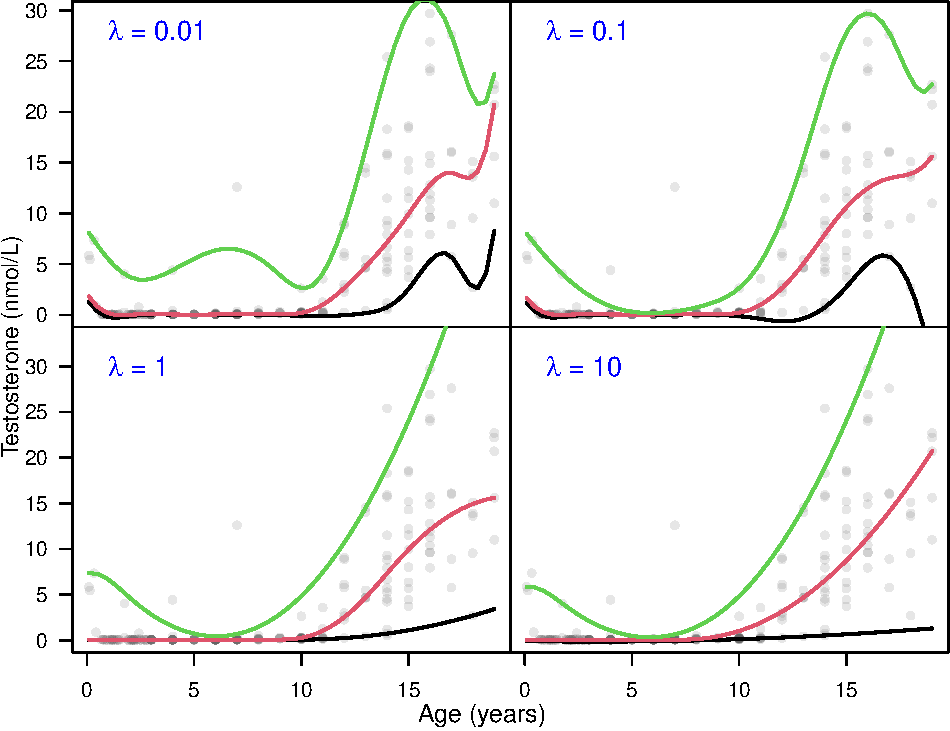
\includegraphics{smoothingfig1-1} \caption{\label{fig:fig1}Comparison of different smoothing values ($\lambda$) for continuous reference interval curves for T in males. Upper curve (green) is 97.5th, median (red), and lower 2.5th (black).}\label{fig:smoothingfig1}
\end{figure}

Instead of manually picking \(\lambda\), in the \texttt{ps()} function
above, we provided a sequence of numbers, coded as:
\texttt{lambda\ =\ lseq(0.01,\ 30,\ l=20)}, which is a logarithmic
sequence of numbers from 0.01 to 30 of length 20
(0.01,0.015,0.023\ldots30). By providing \texttt{ps()} this sequence of
numbers, the \texttt{gcrq} fitting function will calculate the T vs.~age
curve for all those \(\lambda\) smoothing values and identify the
optimum (smoothest curve that still passes closest to the points) using
cross-validation. In the cross-validation, the curve is calculated using
a subset of data points and the accuracy of the fit of the left out
points is assessed iteratively. Using cross-validation, the optimum
\(\lambda\) value for T in males was 0.14.

While cross-validation selects an optimum based on error residuals,
complete automation is seldom perfect and it is appropriate to visually
inspect the results and use our knowledge of the expected data shape to
hone the smoothing parameter. Specifically, we know what the reference
values are in adults and should use that knowledge to tune the fit if
necessary. To improve the fit at the tails (age \textless1 y and
\textgreater18 y), the final smoothing parameter (\(\lambda\)) was
adjusted manually from the initial values based on visual inspection of
the curve -- see supplemental table 1. While this is subjective, it was
determined with relative ease because we started with an optimal value
of the cross-validation.

For completeness, the above description is one way to do the
cross-validation. There are many other ways to do this using the
\textbf{quantregGrowth} package, including defining a penalty matrix,
weighting observations, selecting different types of spline (linear,
quadratic), choosing the exact location of knots, forcing the curve to
continuously increase or decrease, and forcing the curve shape to be
concave-up or concave-down. The interested reader is referred to the
package documentation {[}21,22{]}.

The confidence intervals (95\%) of the fits were determined using the
sandwich formula built into the \textbf{quantregGrowth} package {[}24{]}
but bootstrapping can optionally be selected. Confidence intervals with
shading are plotted using with the code:
\texttt{plot(mm,\ conf.level\ =\ .95,\ shade\ =\ T)}. Negative interval
predictions were rounded to zero. Finally, the manuscript was made
reproducible using the \textbf{renv} package {[}25{]}.

\hypertarget{results}{%
\section{Results}\label{results}}

Continuous intervals were determined for males and females between the
ages of 6 months to 19 years for females (N=195) and 1 month to 19 years
for males (N=226)---see tables \ref{tab:tab1} and \ref{tab:tab2} as well
as figure 2. Intervals were calculated using non-parametric quantile
regression for total T, SHBG, calculated FT and BAT. In both males and
females, T values peaked in the age range of puberty, males being
\(\simeq 10 \times\) higher. SHBG showed varying patterns with age,
differing between males and females.

Confidence intervals were provided for the reference interval estimates,
with higher variability around the tails of the intervals. Predictions
outside the age interval (extrapolation) are not expected to be accurate
given the absence of data.

\begin{figure}[H]
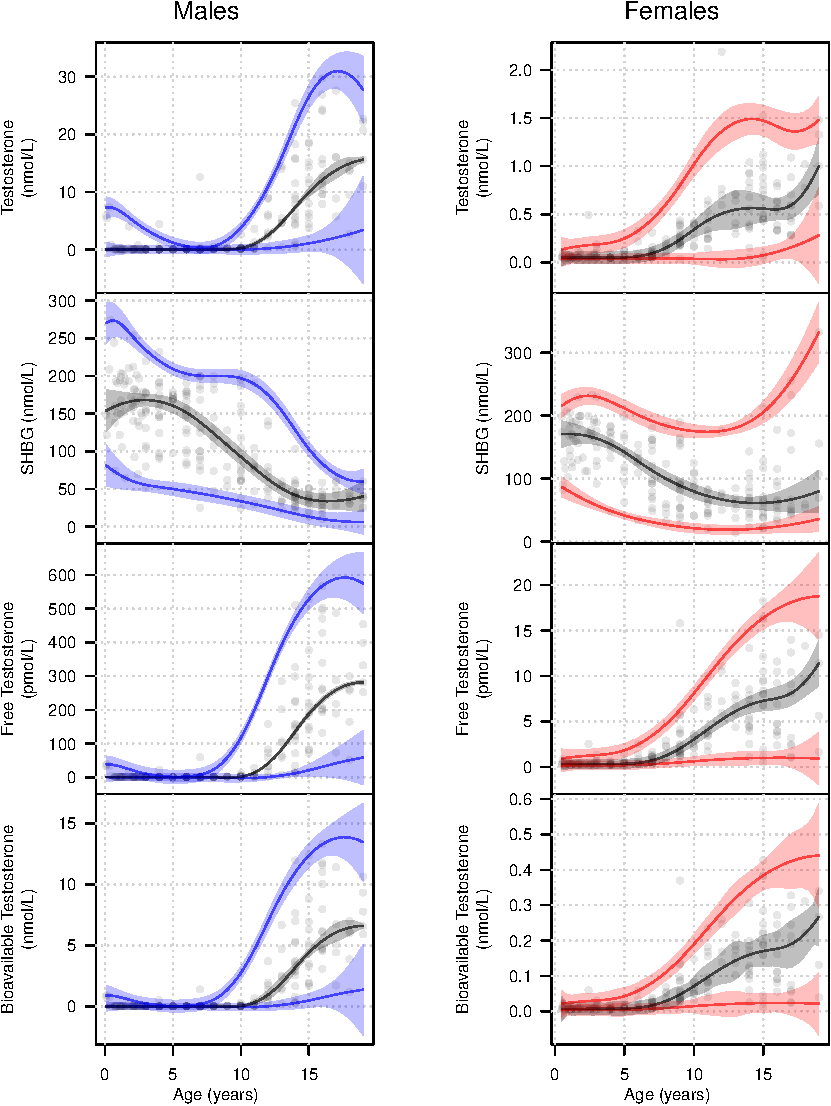
\includegraphics{quantregfitsfig2-1} \caption{\label{fig:fig2}Non-parametric continuous pediatric reference intervals for T, SHBG, BAT and FT in males (left) and females (right) showing confidence intervals calculated using the sandwich formula [15]. The initial optimum and final lambda values are providied in Supplemental Table 1.}\label{fig:quantregfitsfig2}
\end{figure}

\begin{table}[H]

\caption{\label{tab:table1}\label{tab:tab1}Male centile estimates by age in years. Point estimates of the reference intervals are selected at the mid-point of each respective age-bin.}
\centering
\fontsize{7}{9}\selectfont
\begin{tabular}[t]{l>{}r>{}r>{}rrrr>{}r>{}r>{}rrrrr}
\toprule
\multicolumn{1}{c}{ } & \multicolumn{3}{c}{T (nmol/L)} & \multicolumn{3}{c}{SHBG (nmol/L)} & \multicolumn{3}{c}{FT (pmol/L)} & \multicolumn{3}{c}{BAT (nmol/L)} \\
\cmidrule(l{3pt}r{3pt}){2-4} \cmidrule(l{3pt}r{3pt}){5-7} \cmidrule(l{3pt}r{3pt}){8-10} \cmidrule(l{3pt}r{3pt}){11-13}
Age(y) & 2.5th & 50th & 97.5th & 2.5th & 50th & 97.5th & 2.5th & 50th & 97.5th & 2.5th & 50th & 97.5th & N\\
\midrule
0--<1 & \cellcolor[HTML]{ececec}{0.05} & \cellcolor[HTML]{ececec}{0.06} & \cellcolor[HTML]{ececec}{7.31} & 76 & 158 & 274 & \cellcolor[HTML]{ececec}{0.23} & \cellcolor[HTML]{ececec}{0.41} & \cellcolor[HTML]{ececec}{37.73} & 0.01 & 0.01 & 0.88 & 11\\
1--<2 & \cellcolor[HTML]{ececec}{0.04} & \cellcolor[HTML]{ececec}{0.06} & \cellcolor[HTML]{ececec}{6.13} & 65 & 164 & 264 & \cellcolor[HTML]{ececec}{0.16} & \cellcolor[HTML]{ececec}{0.31} & \cellcolor[HTML]{ececec}{28.08} & 0.00 & 0.01 & 0.66 & 17\\
2--<3 & \cellcolor[HTML]{ececec}{0.03} & \cellcolor[HTML]{ececec}{0.05} & \cellcolor[HTML]{ececec}{4.39} & 58 & 168 & 245 & \cellcolor[HTML]{ececec}{0.17} & \cellcolor[HTML]{ececec}{0.26} & \cellcolor[HTML]{ececec}{16.12} & 0.00 & 0.01 & 0.38 & 21\\
3--<4 & \cellcolor[HTML]{ececec}{0.03} & \cellcolor[HTML]{ececec}{0.05} & \cellcolor[HTML]{ececec}{2.93} & 54 & 168 & 228 & \cellcolor[HTML]{ececec}{0.20} & \cellcolor[HTML]{ececec}{0.26} & \cellcolor[HTML]{ececec}{7.47} & 0.00 & 0.01 & 0.18 & 12\\
4--<5 & \cellcolor[HTML]{ececec}{0.03} & \cellcolor[HTML]{ececec}{0.05} & \cellcolor[HTML]{ececec}{1.79} & 51 & 164 & 215 & \cellcolor[HTML]{ececec}{0.22} & \cellcolor[HTML]{ececec}{0.31} & \cellcolor[HTML]{ececec}{2.49} & 0.00 & 0.01 & 0.06 & 14\\
\addlinespace
5--<6 & \cellcolor[HTML]{ececec}{0.04} & \cellcolor[HTML]{ececec}{0.06} & \cellcolor[HTML]{ececec}{0.97} & 49 & 158 & 207 & \cellcolor[HTML]{ececec}{0.17} & \cellcolor[HTML]{ececec}{0.42} & \cellcolor[HTML]{ececec}{1.17} & 0.00 & 0.01 & 0.03 & 9\\
6--<7 & \cellcolor[HTML]{ececec}{0.05} & \cellcolor[HTML]{ececec}{0.07} & \cellcolor[HTML]{ececec}{0.47} & 46 & 147 & 202 & \cellcolor[HTML]{ececec}{0.00} & \cellcolor[HTML]{ececec}{0.57} & \cellcolor[HTML]{ececec}{3.50} & 0.00 & 0.01 & 0.08 & 17\\
7--<8 & \cellcolor[HTML]{ececec}{0.05} & \cellcolor[HTML]{ececec}{0.08} & \cellcolor[HTML]{ececec}{0.34} & 43 & 134 & 200 & \cellcolor[HTML]{ececec}{0.00} & \cellcolor[HTML]{ececec}{0.69} & \cellcolor[HTML]{ececec}{10.97} & 0.00 & 0.02 & 0.26 & 15\\
8--<9 & \cellcolor[HTML]{ececec}{0.04} & \cellcolor[HTML]{ececec}{0.08} & \cellcolor[HTML]{ececec}{0.81} & 40 & 119 & 200 & \cellcolor[HTML]{ececec}{0.00} & \cellcolor[HTML]{ececec}{0.31} & \cellcolor[HTML]{ececec}{30.82} & 0.00 & 0.01 & 0.72 & 9\\
9--<10 & \cellcolor[HTML]{ececec}{0.03} & \cellcolor[HTML]{ececec}{0.09} & \cellcolor[HTML]{ececec}{2.15} & 36 & 104 & 199 & \cellcolor[HTML]{ececec}{0.00} & \cellcolor[HTML]{ececec}{0.00} & \cellcolor[HTML]{ececec}{70.97} & 0.00 & 0.00 & 1.66 & 5\\
\addlinespace
10--<11 & \cellcolor[HTML]{ececec}{0.05} & \cellcolor[HTML]{ececec}{0.37} & \cellcolor[HTML]{ececec}{4.42} & 33 & 89 & 196 & \cellcolor[HTML]{ececec}{0.00} & \cellcolor[HTML]{ececec}{3.24} & \cellcolor[HTML]{ececec}{133.85} & 0.00 & 0.08 & 3.14 & 17\\
11--<12 & \cellcolor[HTML]{ececec}{0.11} & \cellcolor[HTML]{ececec}{1.25} & \cellcolor[HTML]{ececec}{7.63} & 29 & 74 & 187 & \cellcolor[HTML]{ececec}{0.00} & \cellcolor[HTML]{ececec}{18.14} & \cellcolor[HTML]{ececec}{218.80} & 0.00 & 0.43 & 5.13 & 8\\
12--<13 & \cellcolor[HTML]{ececec}{0.26} & \cellcolor[HTML]{ececec}{2.85} & \cellcolor[HTML]{ececec}{11.77} & 25 & 61 & 172 & \cellcolor[HTML]{ececec}{1.38} & \cellcolor[HTML]{ececec}{47.17} & \cellcolor[HTML]{ececec}{315.17} & 0.03 & 1.11 & 7.39 & 8\\
13--<14 & \cellcolor[HTML]{ececec}{0.48} & \cellcolor[HTML]{ececec}{5.08} & \cellcolor[HTML]{ececec}{16.85} & 21 & 49 & 150 & \cellcolor[HTML]{ececec}{6.25} & \cellcolor[HTML]{ececec}{90.28} & \cellcolor[HTML]{ececec}{404.93} & 0.15 & 2.12 & 9.49 & 7\\
14--<15 & \cellcolor[HTML]{ececec}{0.77} & \cellcolor[HTML]{ececec}{7.67} & \cellcolor[HTML]{ececec}{22.30} & 16 & 41 & 125 & \cellcolor[HTML]{ececec}{13.02} & \cellcolor[HTML]{ececec}{142.45} & \cellcolor[HTML]{ececec}{477.60} & 0.31 & 3.34 & 11.19 & 16\\
\addlinespace
15--<16 & \cellcolor[HTML]{ececec}{1.14} & \cellcolor[HTML]{ececec}{10.18} & \cellcolor[HTML]{ececec}{26.94} & 13 & 36 & 101 & \cellcolor[HTML]{ececec}{21.71} & \cellcolor[HTML]{ececec}{192.42} & \cellcolor[HTML]{ececec}{532.51} & 0.51 & 4.51 & 12.48 & 12\\
16--<17 & \cellcolor[HTML]{ececec}{1.59} & \cellcolor[HTML]{ececec}{12.24} & \cellcolor[HTML]{ececec}{29.87} & 10 & 34 & 82 & \cellcolor[HTML]{ececec}{31.85} & \cellcolor[HTML]{ececec}{231.87} & \cellcolor[HTML]{ececec}{569.68} & 0.75 & 5.43 & 13.35 & 13\\
17--<18 & \cellcolor[HTML]{ececec}{2.12} & \cellcolor[HTML]{ececec}{13.84} & \cellcolor[HTML]{ececec}{30.97} & 8 & 34 & 69 & \cellcolor[HTML]{ececec}{42.07} & \cellcolor[HTML]{ececec}{259.83} & \cellcolor[HTML]{ececec}{589.09} & 0.99 & 6.09 & 13.81 & 5\\
18--<19 & \cellcolor[HTML]{ececec}{2.72} & \cellcolor[HTML]{ececec}{14.96} & \cellcolor[HTML]{ececec}{30.26} & 6 & 36 & 62 & \cellcolor[HTML]{ececec}{51.08} & \cellcolor[HTML]{ececec}{276.29} & \cellcolor[HTML]{ececec}{590.75} & 1.20 & 6.47 & 13.84 & 5\\
19--<20 & \cellcolor[HTML]{ececec}{3.40} & \cellcolor[HTML]{ececec}{15.60} & \cellcolor[HTML]{ececec}{27.72} & 6 & 40 & 60 & \cellcolor[HTML]{ececec}{58.64} & \cellcolor[HTML]{ececec}{281.25} & \cellcolor[HTML]{ececec}{574.67} & 1.37 & 6.59 & 13.47 & 5\\
\bottomrule
\end{tabular}
\end{table}

\begin{table}[H]

\caption{\label{tab:table2}\label{tab:tab2}Female centile estimates by age in years.  Point estimates of the reference intervals are selected at the mid-point of each respective age-bin.}
\centering
\fontsize{7}{9}\selectfont
\begin{tabular}[t]{l>{}r>{}r>{}rrrr>{}r>{}r>{}rrrrr}
\toprule
\multicolumn{1}{c}{ } & \multicolumn{3}{c}{T (nmol/L)} & \multicolumn{3}{c}{SHBG (nmol/L)} & \multicolumn{3}{c}{FT (pmol/L)} & \multicolumn{3}{c}{BAT (nmol/L)} \\
\cmidrule(l{3pt}r{3pt}){2-4} \cmidrule(l{3pt}r{3pt}){5-7} \cmidrule(l{3pt}r{3pt}){8-10} \cmidrule(l{3pt}r{3pt}){11-13}
Age(y) & 2.5th & 50th & 97.5th & 2.5th & 50th & 97.5th & 2.5th & 50th & 97.5th & 2.5th & 50th & 97.5th & N\\
\midrule
0--<1 & \cellcolor[HTML]{ececec}{0.04} & \cellcolor[HTML]{ececec}{0.05} & \cellcolor[HTML]{ececec}{0.14} & 83 & 162 & 207 & \cellcolor[HTML]{ececec}{0.18} & \cellcolor[HTML]{ececec}{0.30} & \cellcolor[HTML]{ececec}{0.93} & 0.00 & 0.01 & 0.02 & 8\\
1--<2 & \cellcolor[HTML]{ececec}{0.03} & \cellcolor[HTML]{ececec}{0.05} & \cellcolor[HTML]{ececec}{0.16} & 71 & 171 & 227 & \cellcolor[HTML]{ececec}{0.15} & \cellcolor[HTML]{ececec}{0.30} & \cellcolor[HTML]{ececec}{1.11} & 0.00 & 0.01 & 0.03 & 21\\
2--<3 & \cellcolor[HTML]{ececec}{0.03} & \cellcolor[HTML]{ececec}{0.05} & \cellcolor[HTML]{ececec}{0.18} & 61 & 172 & 234 & \cellcolor[HTML]{ececec}{0.13} & \cellcolor[HTML]{ececec}{0.30} & \cellcolor[HTML]{ececec}{1.24} & 0.00 & 0.01 & 0.03 & 12\\
3--<4 & \cellcolor[HTML]{ececec}{0.03} & \cellcolor[HTML]{ececec}{0.05} & \cellcolor[HTML]{ececec}{0.19} & 53 & 165 & 229 & \cellcolor[HTML]{ececec}{0.13} & \cellcolor[HTML]{ececec}{0.31} & \cellcolor[HTML]{ececec}{1.35} & 0.00 & 0.01 & 0.03 & 7\\
4--<5 & \cellcolor[HTML]{ececec}{0.04} & \cellcolor[HTML]{ececec}{0.05} & \cellcolor[HTML]{ececec}{0.22} & 46 & 153 & 217 & \cellcolor[HTML]{ececec}{0.15} & \cellcolor[HTML]{ececec}{0.33} & \cellcolor[HTML]{ececec}{1.57} & 0.00 & 0.01 & 0.04 & 10\\
\addlinespace
5--<6 & \cellcolor[HTML]{ececec}{0.04} & \cellcolor[HTML]{ececec}{0.05} & \cellcolor[HTML]{ececec}{0.27} & 42 & 137 & 206 & \cellcolor[HTML]{ececec}{0.19} & \cellcolor[HTML]{ececec}{0.36} & \cellcolor[HTML]{ececec}{2.03} & 0.00 & 0.01 & 0.05 & 8\\
6--<7 & \cellcolor[HTML]{ececec}{0.04} & \cellcolor[HTML]{ececec}{0.07} & \cellcolor[HTML]{ececec}{0.37} & 38 & 119 & 196 & \cellcolor[HTML]{ececec}{0.25} & \cellcolor[HTML]{ececec}{0.50} & \cellcolor[HTML]{ececec}{2.78} & 0.01 & 0.01 & 0.07 & 7\\
7--<8 & \cellcolor[HTML]{ececec}{0.04} & \cellcolor[HTML]{ececec}{0.11} & \cellcolor[HTML]{ececec}{0.49} & 34 & 104 & 189 & \cellcolor[HTML]{ececec}{0.32} & \cellcolor[HTML]{ececec}{0.85} & \cellcolor[HTML]{ececec}{3.81} & 0.01 & 0.02 & 0.09 & 16\\
8--<9 & \cellcolor[HTML]{ececec}{0.04} & \cellcolor[HTML]{ececec}{0.17} & \cellcolor[HTML]{ececec}{0.66} & 30 & 91 & 182 & \cellcolor[HTML]{ececec}{0.42} & \cellcolor[HTML]{ececec}{1.44} & \cellcolor[HTML]{ececec}{5.13} & 0.01 & 0.03 & 0.12 & 6\\
9--<10 & \cellcolor[HTML]{ececec}{0.04} & \cellcolor[HTML]{ececec}{0.26} & \cellcolor[HTML]{ececec}{0.86} & 27 & 80 & 178 & \cellcolor[HTML]{ececec}{0.53} & \cellcolor[HTML]{ececec}{2.27} & \cellcolor[HTML]{ececec}{6.72} & 0.01 & 0.05 & 0.16 & 18\\
\addlinespace
10--<11 & \cellcolor[HTML]{ececec}{0.04} & \cellcolor[HTML]{ececec}{0.36} & \cellcolor[HTML]{ececec}{1.07} & 23 & 73 & 176 & \cellcolor[HTML]{ececec}{0.64} & \cellcolor[HTML]{ececec}{3.27} & \cellcolor[HTML]{ececec}{8.53} & 0.02 & 0.08 & 0.20 & 8\\
11--<12 & \cellcolor[HTML]{ececec}{0.03} & \cellcolor[HTML]{ececec}{0.45} & \cellcolor[HTML]{ececec}{1.25} & 19 & 68 & 175 & \cellcolor[HTML]{ececec}{0.75} & \cellcolor[HTML]{ececec}{4.35} & \cellcolor[HTML]{ececec}{10.40} & 0.02 & 0.10 & 0.24 & 10\\
12--<13 & \cellcolor[HTML]{ececec}{0.03} & \cellcolor[HTML]{ececec}{0.52} & \cellcolor[HTML]{ececec}{1.38} & 16 & 65 & 176 & \cellcolor[HTML]{ececec}{0.84} & \cellcolor[HTML]{ececec}{5.37} & \cellcolor[HTML]{ececec}{12.23} & 0.02 & 0.13 & 0.29 & 4\\
13--<14 & \cellcolor[HTML]{ececec}{0.04} & \cellcolor[HTML]{ececec}{0.55} & \cellcolor[HTML]{ececec}{1.46} & 14 & 63 & 182 & \cellcolor[HTML]{ececec}{0.91} & \cellcolor[HTML]{ececec}{6.24} & \cellcolor[HTML]{ececec}{13.89} & 0.02 & 0.15 & 0.33 & 6\\
14--<15 & \cellcolor[HTML]{ececec}{0.05} & \cellcolor[HTML]{ececec}{0.56} & \cellcolor[HTML]{ececec}{1.49} & 17 & 62 & 193 & \cellcolor[HTML]{ececec}{0.96} & \cellcolor[HTML]{ececec}{6.89} & \cellcolor[HTML]{ececec}{15.32} & 0.02 & 0.16 & 0.36 & 13\\
\addlinespace
15--<16 & \cellcolor[HTML]{ececec}{0.08} & \cellcolor[HTML]{ececec}{0.56} & \cellcolor[HTML]{ececec}{1.47} & 22 & 61 & 209 & \cellcolor[HTML]{ececec}{0.99} & \cellcolor[HTML]{ececec}{7.29} & \cellcolor[HTML]{ececec}{16.50} & 0.02 & 0.17 & 0.39 & 15\\
16--<17 & \cellcolor[HTML]{ececec}{0.11} & \cellcolor[HTML]{ececec}{0.55} & \cellcolor[HTML]{ececec}{1.41} & 30 & 62 & 230 & \cellcolor[HTML]{ececec}{1.00} & \cellcolor[HTML]{ececec}{7.57} & \cellcolor[HTML]{ececec}{17.44} & 0.02 & 0.18 & 0.41 & 10\\
17--<18 & \cellcolor[HTML]{ececec}{0.16} & \cellcolor[HTML]{ececec}{0.60} & \cellcolor[HTML]{ececec}{1.36} & 41 & 67 & 257 & \cellcolor[HTML]{ececec}{1.00} & \cellcolor[HTML]{ececec}{8.14} & \cellcolor[HTML]{ececec}{18.13} & 0.02 & 0.19 & 0.43 & 10\\
18--<19 & \cellcolor[HTML]{ececec}{0.21} & \cellcolor[HTML]{ececec}{0.74} & \cellcolor[HTML]{ececec}{1.38} & 54 & 83 & 292 & \cellcolor[HTML]{ececec}{0.97} & \cellcolor[HTML]{ececec}{9.38} & \cellcolor[HTML]{ececec}{18.58} & 0.02 & 0.22 & 0.44 & 2\\
19--<20 & \cellcolor[HTML]{ececec}{0.28} & \cellcolor[HTML]{ececec}{1.00} & \cellcolor[HTML]{ececec}{1.48} & 69 & 108 & 333 & \cellcolor[HTML]{ececec}{0.92} & \cellcolor[HTML]{ececec}{11.38} & \cellcolor[HTML]{ececec}{18.78} & 0.02 & 0.27 & 0.44 & 4\\
\bottomrule
\end{tabular}
\end{table}

\hypertarget{discussion}{%
\section{Discussion}\label{discussion}}

We have demonstrated the process of generating continuous reference
intervals using a pediatric dataset for T, SHBG, FT and calculated BAT
for male and female children under 20 years. Only a few studies have
investigated total T reference intervals using LC-MS/MS in pediatric
populations {[}1,4--7{]}. A graphical comparison of these is shown in
figure 3 showing reasonable agreement among the studies bearing in mind
that the statistical analyses are performed differently and samples are
differentially binned into age-categories. However, figure 3 also
starkly illustrates the problem with binned reference interval studies,
namely, that there are large jumps in the reference intervals seen when
transitioning from one age-bin to the next. Obviously this does not
reflect physiology and would induce misclassification with increasing
frequency as bin sizes grow. For example in both the studies of Soldin
{[}1{]} and Bae {[}7{]}, a large jump of \(\simeq 17-25\) nmol/L is seen
in the upper limit of normal for boys after the age of 10 y and a
similar phenomenon is seen in Kushnir's study {[}5{]}, attenuated
somewhat by the narrower bin sizes.

Of note, concern has been raised about incorrect application of the
Hoffmann indirect method leading to inappropriately narrow reference
intervals {[}26{]}, which would affect the results from Soldin et al,
but the material effect of this error is hard to appreciate in figure 3.

\begin{figure}[H]
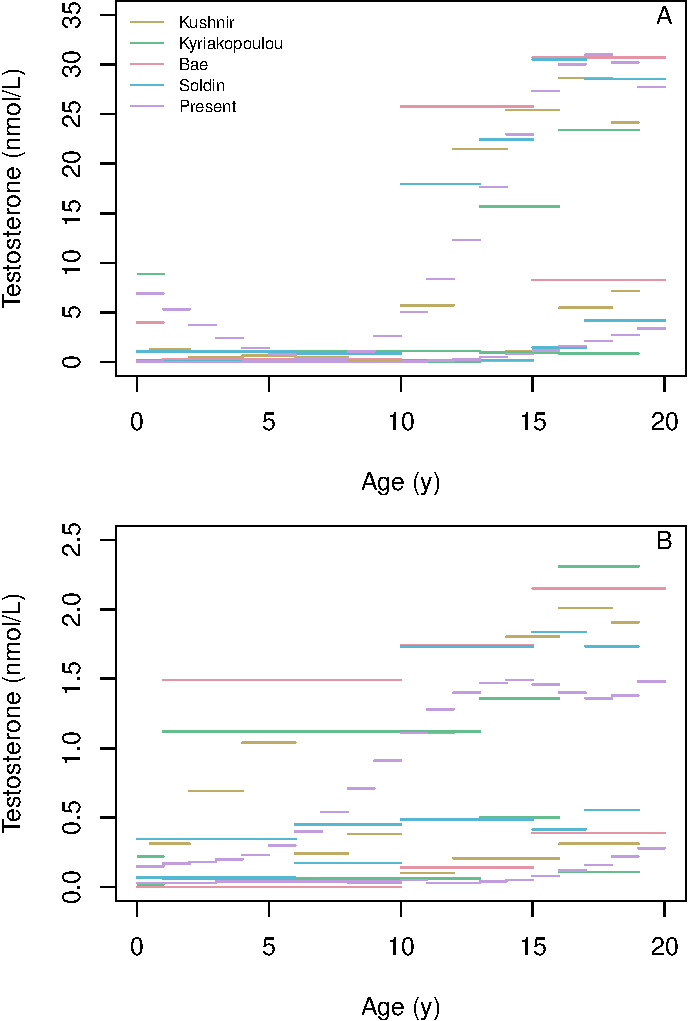
\includegraphics{comparisonfig3-1} \caption{\label{fig:fig3}A graphical comparison of reference intervals for total tesotsterone by LC-MS/MS from various studies for male (A) and female (B) children. Lower and upper reference intervals for a given study are shown as horizontal lines.}\label{fig:comparisonfig3}
\end{figure}

A weakness of the present study in comparison to others is the relative
dearth of subjects in the age-category of 0--12 months (N=8 F and N=11
M) which means that subjects demonstrating the phenomenon of
mini-puberty {[}27{]} are few. While we do see elevated T for males in
this age-category, we do not see them in our female data, similar to
Kyriakopoulou et al.~However, Bae et al do have a large number of female
subjects less than 1 year of age showing increased T levels as does a
subsequent study from the same group as Kyriakopoulou et al {[}28{]}
using Roche Cobas 8000 for both T and SHBG. The phenomenon of
mini-puberty is a potential hazard in continuous fitting algorithms
because the age window where mini-puberty occurs is so narrow and the
androgen concentrations so high that the modeled centile functions may
have a shallower slope than is required to accurately reflect
physiology. In this context, a dedicated (i.e.~binned) analysis of
results for patients less than 1 year of age may be warranted.

Another weakness of this study is that androgen and SHBG concentration
is dependent on Tanner Stage for pubescent males and females and are
also affected by phase of the menstrual cycle and/or the use of oral
contraceptives. Given the anonymity of the specimens, this information
was not available.

This study has also not taken into account the fact that median albumin
concentrations by age are not fixed at 43 g/L throughout life but show
age-dependence, being lower in early childhood--especially in the
neonatal period and in children under 4 years {[}29{]}. While we
acknowledge this, attempts to address it would not have practical
impact. The Vermeulen equation itself is really a \emph{metric} of FT
calculated by means of mass-action using estimates of the binding
coefficients of albumin and SHBG from studies now quite old {[}30{]} and
estimates of FT and BAT are not strongly affected by albumin
concentration. In this sense, we make the assumption that if the
reference intervals are determined with the same albumin estimates as
the patient, then results will be interpretable, though not applicable
to other analytical methodologies.

Pediatric reference intervals for SHBG using the Roche Cobas e411 and
e601 methods have been reported previously {[}28,31{]} though our
results can only be superficially compared because of differences in
biochemical and statistical analysis. Zec et al only provide reference
interval results for children aged 1--10 y and obtain results of
22.7--166.5 nmol/L for females and 21.5--186.2 nmol/L for boys. While
these do not seem incompatible with the present study, detailed
comparison is not possible. The more recent study from the CALIPER group
{[}28{]} is also difficult to compare because samples \(>200\) nmol/L
were not diluted and re-run so as to obtain a numerical result--all
results \(>200\) are replaced with 200.

We are not aware of FT or BAT pediatric reference interval studies using
LC-MS/MS for the T measurement, though results for the Roche Cobas e411
{[}31{]} and Abbott Architect ci4100 are reported {[}32{]}.

A limitation of continuous reference intervals (and fitting any models
with tuneable parameters) is the subjectivity of selection of the
parameters. In this manuscript the initial `smoothing' parameter
\(\lambda\) was sub-optimal based on visual inspection. As a result most
of these were subjectively manually chosen based on the `best' appearing
curve (no sharp increase or decreases in the tail age groups that were
inconsistent with known effects of age). By comparison, parametric and
non-parametric methods don't have smoothing options and avoid the
problem, but conversely suffer subjectivity in the selection of age
partitions themselves.

The strength of this study, and continuous reference intervals in
general, is that we did not need to make any assumptions or arbitrary
age partitions. Non-parametric continuous intervals use all the data,
are robust to outliers, and avoid large jumps between intervals at
puberty. Another advantage of continuous intervals is the ability to
calculate point estimates for any age using the curve model. For
example, the lower, median, and upper limits for T in a female aged
14.5, is determine with the code:
\texttt{round(predict(fm,\ newdata\ =\ data.frame(age=14.5)),2)},
yielding: 0.06, 0.56, 1.49; the model is \texttt{fm}, we add our age of
interest as a \texttt{data.frame} and surround the call with
\texttt{round} to get 2 decimal places (as opposed to the default 8).
This can be helpful in challenging cases and part of the discussion with
a clinician. Such models may also be shared as web applications
(e.g.~RShiny {[}33{]}) to allow users to generate point estimates
themselves. Though it not possible to implement fully continuous
age-dependent reference intervals into a laboratory information system,
point estimates naturally permit reference interval estimates that are
as granular as month-by-month or year-by-year.

\hypertarget{conclusion}{%
\section{Conclusion}\label{conclusion}}

In this study, we demonstrated the calculation of continuous reference
intervals for T, SHBG, and calculated free and biovailable T in males
and females under the age of 20 using the \textbf{quantregGrowth}
package. Reference intervals are an essential tool against which to
evaluate results of individual patients for clinical decision-making.
Continuous reference intervals are a superior method for determining
intervals where values vary with age. Continuous intervals avoid
problems with arbitrary age partitions, sharp differences between age
group, and data sparsity. In, particular non-parametric methods have
advantages in using all of the data (rather than age partitions), do not
require arbitrary removal of outliers, and are resistant to asymmetric,
non-normality, and heteroscedastic data {[}22{]}. We attempted to
describe the process of generating such intervals in a reproducible way
such that readers could derive their own continuous intervals for this
or other analytes. The RMarkdown source code and raw data for this paper
can be downloaded at
\url{https://github.com/drdanholmes/jmsacl_continuous_reference_interval}
and in the supplementary material.

\hypertarget{conflicts-of-interest}{%
\section{Conflicts of Interest}\label{conflicts-of-interest}}

The authors have no relevant conflicts of interest to disclose.

\hypertarget{supplemental-data}{%
\section{Supplemental Data}\label{supplemental-data}}

\begin{table}[]
\caption*{Supplemental Table 1: Initial and final smoothing ($\lambda$) values. The reader will note that the initial value of the $\lambda$ parameter was more than $10\times$ the final value for female T, in contrast to the initial values for the other parameters which are on the same order of magnitude as their final values. This is because the cross-validation score for the fit did not improve appreciably for values of $\lambda$ between about 0.7 and 30.  Howevever, the larger values of $\lambda$ result in underfitting, justifying the selection of a lower value resulting in a less restrictive fit. Ultimately, this is a judgement call. }
\label{tab:my-table}
\begin{tabular}{l|llll}
                          & \multicolumn{2}{l}{Male $\lambda$} & \multicolumn{2}{l}{Female $\lambda$} \\ \cline{2-5} 
Hormone                   & Initial       & Final          & Initial        & Final            \\ \hline
T                         & 0.19           & 0.4            & 12.9          & 0.7              \\
BAT                       & 0.08           & 0.6            & 0.08          & 0.6              \\
FT                        & 0.08           & 0.6            & 0.08          & 0.6              \\
SHBG                      & 0.08           & 0.08           & 0.12          & 0.12       
\end{tabular}
\end{table}

\hypertarget{references}{%
\section*{References}\label{references}}
\addcontentsline{toc}{section}{References}

\hypertarget{refs}{}
\begin{CSLReferences}{0}{0}
\leavevmode\hypertarget{ref-soldin2009pediatric}{}%
\CSLLeftMargin{{[}1{]} }
\CSLRightInline{O.P. Soldin, H. Sharma, L. Husted, S.J. Soldin,
Pediatric reference intervals for aldosterone,
17\(\alpha\)-hydroxyprogesterone, dehydroepiandrosterone, testosterone
and 25-hydroxy vitamin D3 using tandem mass spectrometry, Clinical
Biochemistry. 42 (2009) 823--827.}

\leavevmode\hypertarget{ref-konforte2013complex}{}%
\CSLLeftMargin{{[}2{]} }
\CSLRightInline{D. Konforte, J.L. Shea, L. Kyriakopoulou, D. Colantonio,
A.H. Cohen, J. Shaw, D. Bailey, M.K. Chan, D. Armbruster, K. Adeli,
Complex biological pattern of fertility hormones in children and
adolescents: A study of healthy children from the CALIPER cohort and
establishment of pediatric reference intervals, Clinical Chemistry. 59
(2013) 1215--1227.}

\leavevmode\hypertarget{ref-greaves2015hormone}{}%
\CSLLeftMargin{{[}3{]} }
\CSLRightInline{R.F. Greaves, J. Pitkin, C.S. Ho, J. Baglin, R.W. Hunt,
M.R. Zacharin, Hormone modeling in preterm neonates: Establishment of
pituitary and steroid hormone reference intervals, The Journal of
Clinical Endocrinology \& Metabolism. 100 (2015) 1097--1103.}

\leavevmode\hypertarget{ref-kulle2010novel}{}%
\CSLLeftMargin{{[}4{]} }
\CSLRightInline{A. Kulle, F.G. Riepe, D. Melchior, O. Hiort, P.
Holterhus, A novel ultrapressure liquid chromatography tandem mass
spectrometry method for the simultaneous determination of
androstenedione, testosterone, and dihydrotestosterone in pediatric
blood samples: Age-and sex-specific reference data, The Journal of
Clinical Endocrinology \& Metabolism. 95 (2010) 2399--2409.}

\leavevmode\hypertarget{ref-kushnir2010liquid}{}%
\CSLLeftMargin{{[}5{]} }
\CSLRightInline{M.M. Kushnir, T. Blamires, A.L. Rockwood, W.L. Roberts,
B. Yue, E. Erdogan, A.M. Bunker, A.W. Meikle, Liquid
chromatography--tandem mass spectrometry assay for androstenedione,
dehydroepiandrosterone, and testosterone with pediatric and adult
reference intervals, Clinical Chemistry. 56 (2010) 1138--1147.}

\leavevmode\hypertarget{ref-kyriakopoulou2013sensitive}{}%
\CSLLeftMargin{{[}6{]} }
\CSLRightInline{L. Kyriakopoulou, M. Yazdanpanah, D. Colantonio, M.
Chan, C. Daly, K. Adeli, A sensitive and rapid mass spectrometric method
for the simultaneous measurement of eight steroid hormones and CALIPER
pediatric reference intervals, Clinical Biochemistry. 46 (2013)
642--651.}

\leavevmode\hypertarget{ref-bae2019reference}{}%
\CSLLeftMargin{{[}7{]} }
\CSLRightInline{Y.J. Bae, R. Zeidler, R. Baber, M. Vogel, K. Wirkner, M.
Loeffler, U. Ceglarek, W. Kiess, A. Körner, J. Thiery, others, Reference
intervals of nine steroid hormones over the life-span analyzed by
LC-MS/MS: Effect of age, gender, puberty, and oral contraceptives, The
Journal of Steroid Biochemistry and Molecular Biology. 193 (2019)
105409.}

\leavevmode\hypertarget{ref-healy1974notes}{}%
\CSLLeftMargin{{[}8{]} }
\CSLRightInline{M. Healy, Notes on the statistics of growth standards,
Annals of Human Biology. 1 (1974) 41--46.}

\leavevmode\hypertarget{ref-cole1992smoothing}{}%
\CSLLeftMargin{{[}9{]} }
\CSLRightInline{T.J. Cole, P.J. Green, Smoothing reference centile
curves: The LMS method and penalized likelihood, Statistics in Medicine.
11 (1992) 1305--1319.}

\leavevmode\hypertarget{ref-royston1994regression}{}%
\CSLLeftMargin{{[}10{]} }
\CSLRightInline{P. Royston, D.G. Altman, Regression using fractional
polynomials of continuous covariates: Parsimonious parametric modelling,
Journal of the Royal Statistical Society: Series C (Applied Statistics).
43 (1994) 429--453.}

\leavevmode\hypertarget{ref-rigby2005generalized}{}%
\CSLLeftMargin{{[}11{]} }
\CSLRightInline{R.A. Rigby, D.M. Stasinopoulos, Generalized additive
models for location, scale and shape, Journal of the Royal Statistical
Society: Series C (Applied Statistics). 54 (2005) 507--554.}

\leavevmode\hypertarget{ref-koenker_2005}{}%
\CSLLeftMargin{{[}12{]} }
\CSLRightInline{R. Koenker, Quantile regression, Cambridge University
Press, 2005. \url{https://doi.org/10.1017/CBO9780511754098}.}

\leavevmode\hypertarget{ref-muggeo2013estimating}{}%
\CSLLeftMargin{{[}13{]} }
\CSLRightInline{V.M. Muggeo, M. Sciandra, A. Tomasello, S. Calvo,
Estimating growth charts via nonparametric quantile regression: A
practical framework with application in ecology, Environmental and
Ecological Statistics. 20 (2013) 519--531.}

\leavevmode\hypertarget{ref-muggeo2020multiple}{}%
\CSLLeftMargin{{[}14{]} }
\CSLRightInline{V.M. Muggeo, F. Torretta, P.H. Eilers, M. Sciandra, M.
Attanasio, Multiple smoothing parameters selection in additive
regression quantiles, Statistical Modelling. (2020) 1471082X20929802.}

\leavevmode\hypertarget{ref-quantreggrowth}{}%
\CSLLeftMargin{{[}15{]} }
\CSLRightInline{V.M. Muggeo, quantregGrowth: Growth charts via smooth
regression quantiles with automatic smoothness estimation and additive
terms, (2021 (accessed July 7, 2021)).}

\leavevmode\hypertarget{ref-gislefoss2009stability}{}%
\CSLLeftMargin{{[}16{]} }
\CSLRightInline{R.E. Gislefoss, T.K. Grimsrud, L. Mørkrid, Stability of
selected serum proteins after long-term storage in the janus serum bank,
Clinical Chemistry and Laboratory Medicine. 47 (2009) 596--603.}

\leavevmode\hypertarget{ref-handelsman2020circulating}{}%
\CSLLeftMargin{{[}17{]} }
\CSLRightInline{D. Handelsman, R. Desai, M. Seibel, D. Le Couteur, R.
Cumming, Circulating sex steroid measurements of men by mass
spectrometry are highly reproducible after prolonged frozen storage, The
Journal of Steroid Biochemistry and Molecular Biology. 197 (2020)
105528.}

\leavevmode\hypertarget{ref-french2013development}{}%
\CSLLeftMargin{{[}18{]} }
\CSLRightInline{D. French, Development and validation of a serum total
testosterone liquid chromatography--tandem mass spectrometry (LC--MS/MS)
assay calibrated to NIST SRM 971, Clinica Chimica Acta. 415 (2013)
109--117.}

\leavevmode\hypertarget{ref-french2019comparison}{}%
\CSLLeftMargin{{[}19{]} }
\CSLRightInline{D. French, J. Drees, J.A. Stone, D.T. Holmes, J.G. van
der Gugten, Comparison of four clinically validated testosterone
LC-MS/MS assays: Harmonization is an attainable goal, Clinical Mass
Spectrometry. 11 (2019) 12--20.}

\leavevmode\hypertarget{ref-de2006calculation}{}%
\CSLLeftMargin{{[}20{]} }
\CSLRightInline{W. De Ronde, Y.T. Van Der Schouw, H.A. Pols, L.J.
Gooren, M. Muller, D.E. Grobbee, F.H. De Jong, Calculation of
bioavailable and free testosterone in men: A comparison of 5 published
algorithms, Clinical Chemistry. 52 (2006) 1777--1784.}

\leavevmode\hypertarget{ref-quantreg1}{}%
\CSLLeftMargin{{[}21{]} }
\CSLRightInline{V.M.R. Muggeo, F. Torretta, P.H.C. Eilers, M. Sciandra,
M. Attanasio, Multiple smoothing parameters selection in additive
regression quantiles, Statistical Modelling. 0 1471082X20929802.
\url{https://doi.org/10.1177/1471082X20929802}.}

\leavevmode\hypertarget{ref-quantreg2}{}%
\CSLLeftMargin{{[}22{]} }
\CSLRightInline{V.M. Muggeo, M. Sciandra, A. Tomasello, S. Calvo,
Estimating growth charts via nonparametric quantile regression: A
practical framework with application in ecology, Environmental and
Ecological Statistics. 20 (2013) 519--531.}

\leavevmode\hypertarget{ref-asgari_continuous_2019}{}%
\CSLLeftMargin{{[}23{]} }
\CSLRightInline{S. Asgari, V. Higgins, C. McCudden, K. Adeli, Continuous
reference intervals for 38 biochemical markers in healthy children and
adolescents: Comparisons to traditionally partitioned reference
intervals, Clinical Biochemistry. 73 (2019) 82--89.}

\leavevmode\hypertarget{ref-hardin2003sandwich}{}%
\CSLLeftMargin{{[}24{]} }
\CSLRightInline{J.W. Hardin, The sandwich estimate of variance, in:
Maximum Likelihood Estimation of Misspecified Models: Twenty Years
Later, Emerald Group Publishing Limited, 2003.}

\leavevmode\hypertarget{ref-renvpackage}{}%
\CSLLeftMargin{{[}25{]} }
\CSLRightInline{K. Ushey, Renv: Project environments, 2021.
\url{https://CRAN.R-project.org/package=renv}.}

\leavevmode\hypertarget{ref-holmes2019widespread}{}%
\CSLLeftMargin{{[}26{]} }
\CSLRightInline{D.T. Holmes, K.A. Buhr, Widespread incorrect
implementation of the hoffmann method, the correct approach, and modern
alternatives, American Journal of Clinical Pathology. 151 (2019)
328--336.}

\leavevmode\hypertarget{ref-forest1973evidence}{}%
\CSLLeftMargin{{[}27{]} }
\CSLRightInline{M.G. Forest, A.M. Cathiard, J.A. Bertrand, Evidence of
testicular activity in early infancy, The Journal of Clinical
Endocrinology \& Metabolism. 37 (1973) 148--151.}

\leavevmode\hypertarget{ref-bohn2019paediatric}{}%
\CSLLeftMargin{{[}28{]} }
\CSLRightInline{M.K. Bohn, V. Higgins, S. Asgari, F. Leung, B. Hoffman,
J. Macri, K. Adeli, Paediatric reference intervals for 17 roche cobas
8000 e602 immunoassays in the CALIPER cohort of healthy children and
adolescents, Clinical Chemistry and Laboratory Medicine (CCLM). 57
(2019) 1968--1979.}

\leavevmode\hypertarget{ref-lockitch1988age}{}%
\CSLLeftMargin{{[}29{]} }
\CSLRightInline{G. Lockitch, A. Halstead, S. Albersheim, C. MacCallum,
G. Quigley, Age-and sex-specific pediatric reference intervals for
biochemistry analytes as measured with the ektachem-700 analyzer.,
Clinical Chemistry. 34 (1988) 1622--1625.}

\leavevmode\hypertarget{ref-vermeulen1971apparent}{}%
\CSLLeftMargin{{[}30{]} }
\CSLRightInline{A. Vermeulen, T. Stoica, L. Verdonck, The apparent free
testosterone concentration, an index of androgenicity, The Journal of
Clinical Endocrinology \& Metabolism. 33 (1971) 759--767.}

\leavevmode\hypertarget{ref-zec2012reference}{}%
\CSLLeftMargin{{[}31{]} }
\CSLRightInline{I. Zec, I. Kučak, I. Begčević, A.-M. Šimundić, D.
Tišlarić-Medenjak, Ž.B. Megla, N. Vrkić, Reference intervals for
reproductive hormones in prepubertal children on the automated roche
cobas e 411 analyzer, Clinical Biochemistry. 45 (2012) 1206--1212.}

\leavevmode\hypertarget{ref-raizman2015pediatric}{}%
\CSLLeftMargin{{[}32{]} }
\CSLRightInline{J.E. Raizman, F. Quinn, D.A. Armbruster, K. Adeli,
Pediatric reference intervals for calculated free testosterone,
bioavailable testosterone and free androgen index in the CALIPER cohort,
Clinical Chemistry and Laboratory Medicine (CCLM). 53 (2015)
e239--e243.}

\leavevmode\hypertarget{ref-shiny}{}%
\CSLLeftMargin{{[}33{]} }
\CSLRightInline{W. Chang, J. Cheng, J. Allaire, C. Sievert, B.
Schloerke, Y. Xie, J. Allen, J. McPherson, A. Dipert, B. Borges, Shiny:
Web application framework for {R}, (2021).
\url{https://CRAN.R-project.org/package=shiny}.}

\end{CSLReferences}


\end{document}

